\begin{filecontents*}[overwrite]{gallery-showcase-bw.tex}
\documentclass[10pt, a4paper, theme = bw]{../main/main}

\usepackage[utf8]{inputenc}
\usepackage[T1]{fontenc}

\usepackage[french]{babel, varioref}

\usepackage{enumitem}
\frenchsetup{StandardItemLabels=true}

\usepackage{tabularray}

\usepackage[lang = french]{tutodoc}


\usepackage{../admonitions/admonitions.cls}
\usepackage{../listing/listing.cls}
\usepackage{../version-n-change/version-n-change.cls}

\newcommand\thisstyle{bw}

\newcommand\myexrmktext{
    \tdocdate{2024-10-23}
    Dans le flot du texte, il est toujours utile de pouvoir indiquer des exemples et des remarques qui viennent compléter le contenu principal.
}

\newcommand\myadmotext{
    \tdocversion{1.6.0}[2024-10-23]
    Suivant le contexte d'utilisation, il est parfois nécessaire de pouvoir mettre en avant des contenus en indiquant leur degré d'importance.
}

\newcommand\myhighlightedtext{
    Que dire
    \footnote{
        N'oublions pas les notes de bas de page...
    } ?
    Je ne sais pas, mais en tout cas, il semble sympathique de montrer ce que peut donner telle mise en forme, ou telle autre. Non ?
}

\begin{document}

{\Huge\bfseries Le thème \texttt{"\thisstyle"}}

\section{Mettre en avant, versionner et dater}

\ExplSyntaxOn

\seq_map_inline:Nn \__g_tutodoc_focus_std_seq {
    \subsection*{tdoc#1}

    \myexrmktext

    \begin{tdoc#1}
        \myhighlightedtext
    \end{tdoc#1}

    \myexrmktext
}

\ifcsundef{__g_tutodoc_focus_color_seq}{
    \prop_map_inline:Nn \__g_tutodoc_focus_color_prop {
        \subsection*{tdoc#1}

        \myadmotext

        \begin{tdoc#1}
            \myhighlightedtext
        \end{tdoc#1}

        \myadmotext
    }
} {
    \seq_map_inline:Nn \__g_tutodoc_focus_color_seq {
        \subsection*{tdoc#1}

        \myadmotext

        \begin{tdoc#1}
            \myhighlightedtext
        \end{tdoc#1}

        \myadmotext
    }
}

\ExplSyntaxOff

\section{Des codes \LaTeX}

Il est indispensable de pouvoir montrer des cas d'utilisation en \LaTeX.

\begin{tdoclatex}
Voir du code \LaTeX\ mis en forme, c'est sympa : $E = m c^2$ ou $\pi \neq \frac{3}{14}$.
\end{tdoclatex}


On dispose aussi d'un mode côte-à-côte moins envahissant. Sympa ! Non ?

\begin{tdoclatex}[sbs]
Voir du code \LaTeX\ mis en forme,
c'est sympa : $E = m c^2$ ou
$\pi \neq \frac{3}{14}$.
\end{tdoclatex}

\end{document}

\end{filecontents*}

\begin{filecontents*}[overwrite]{gallery-showcase-color.tex}
\documentclass[10pt, a4paper, theme = color]{../main/main}

\usepackage[utf8]{inputenc}
\usepackage[T1]{fontenc}

\usepackage[french]{babel, varioref}

\usepackage{enumitem}
\frenchsetup{StandardItemLabels=true}

\usepackage{tabularray}

\usepackage[lang = french]{tutodoc}


\usepackage{../admonitions/admonitions.cls}
\usepackage{../listing/listing.cls}
\usepackage{../version-n-change/version-n-change.cls}

\newcommand\thisstyle{color}

\newcommand\myexrmktext{
    \tdocdate{2024-10-23}
    Dans le flot du texte, il est toujours utile de pouvoir indiquer des exemples et des remarques qui viennent compléter le contenu principal.
}

\newcommand\myadmotext{
    \tdocversion{1.6.0}[2024-10-23]
    Suivant le contexte d'utilisation, il est parfois nécessaire de pouvoir mettre en avant des contenus en indiquant leur degré d'importance.
}

\newcommand\myhighlightedtext{
    Que dire
    \footnote{
        N'oublions pas les notes de bas de page...
    } ?
    Je ne sais pas, mais en tout cas, il semble sympathique de montrer ce que peut donner telle mise en forme, ou telle autre. Non ?
}

\begin{document}

{\Huge\bfseries Le thème \texttt{"\thisstyle"}}

\section{Mettre en avant, versionner et dater}

\ExplSyntaxOn

\seq_map_inline:Nn \__g_tutodoc_focus_std_seq {
    \subsection*{tdoc#1}

    \myexrmktext

    \begin{tdoc#1}
        \myhighlightedtext
    \end{tdoc#1}

    \myexrmktext
}

\ifcsundef{__g_tutodoc_focus_color_seq}{
    \prop_map_inline:Nn \__g_tutodoc_focus_color_prop {
        \subsection*{tdoc#1}

        \myadmotext

        \begin{tdoc#1}
            \myhighlightedtext
        \end{tdoc#1}

        \myadmotext
    }
} {
    \seq_map_inline:Nn \__g_tutodoc_focus_color_seq {
        \subsection*{tdoc#1}

        \myadmotext

        \begin{tdoc#1}
            \myhighlightedtext
        \end{tdoc#1}

        \myadmotext
    }
}

\ExplSyntaxOff

\section{Des codes \LaTeX}

Il est indispensable de pouvoir montrer des cas d'utilisation en \LaTeX.

\begin{tdoclatex}
Voir du code \LaTeX\ mis en forme, c'est sympa : $E = m c^2$ ou $\pi \neq \frac{3}{14}$.
\end{tdoclatex}


On dispose aussi d'un mode côte-à-côte moins envahissant. Sympa ! Non ?

\begin{tdoclatex}[sbs]
Voir du code \LaTeX\ mis en forme,
c'est sympa : $E = m c^2$ ou
$\pi \neq \frac{3}{14}$.
\end{tdoclatex}

\end{document}

\end{filecontents*}

\begin{filecontents*}[overwrite]{gallery-showcase-dark.tex}
\documentclass[10pt, a4paper, theme = dark]{../main/main}

\usepackage[utf8]{inputenc}
\usepackage[T1]{fontenc}

\usepackage[french]{babel, varioref}

\usepackage{enumitem}
\frenchsetup{StandardItemLabels=true}

\usepackage{tabularray}

\usepackage[lang = french]{tutodoc}


\usepackage{../admonitions/admonitions.cls}
\usepackage{../listing/listing.cls}
\usepackage{../version-n-change/version-n-change.cls}

\newcommand\thisstyle{dark}

\newcommand\myexrmktext{
    \tdocdate{2024-10-23}
    Dans le flot du texte, il est toujours utile de pouvoir indiquer des exemples et des remarques qui viennent compléter le contenu principal.
}

\newcommand\myadmotext{
    \tdocversion{1.6.0}[2024-10-23]
    Suivant le contexte d'utilisation, il est parfois nécessaire de pouvoir mettre en avant des contenus en indiquant leur degré d'importance.
}

\newcommand\myhighlightedtext{
    Que dire
    \footnote{
        N'oublions pas les notes de bas de page...
    } ?
    Je ne sais pas, mais en tout cas, il semble sympathique de montrer ce que peut donner telle mise en forme, ou telle autre. Non ?
}

\begin{document}

{\Huge\bfseries Le thème \texttt{"\thisstyle"}}

\section{Mettre en avant, versionner et dater}

\ExplSyntaxOn

\seq_map_inline:Nn \__g_tutodoc_focus_std_seq {
    \subsection*{tdoc#1}

    \myexrmktext

    \begin{tdoc#1}
        \myhighlightedtext
    \end{tdoc#1}

    \myexrmktext
}

\ifcsundef{__g_tutodoc_focus_color_seq}{
    \prop_map_inline:Nn \__g_tutodoc_focus_color_prop {
        \subsection*{tdoc#1}

        \myadmotext

        \begin{tdoc#1}
            \myhighlightedtext
        \end{tdoc#1}

        \myadmotext
    }
} {
    \seq_map_inline:Nn \__g_tutodoc_focus_color_seq {
        \subsection*{tdoc#1}

        \myadmotext

        \begin{tdoc#1}
            \myhighlightedtext
        \end{tdoc#1}

        \myadmotext
    }
}

\ExplSyntaxOff

\section{Des codes \LaTeX}

Il est indispensable de pouvoir montrer des cas d'utilisation en \LaTeX.

\begin{tdoclatex}
Voir du code \LaTeX\ mis en forme, c'est sympa : $E = m c^2$ ou $\pi \neq \frac{3}{14}$.
\end{tdoclatex}


On dispose aussi d'un mode côte-à-côte moins envahissant. Sympa ! Non ?

\begin{tdoclatex}[sbs]
Voir du code \LaTeX\ mis en forme,
c'est sympa : $E = m c^2$ ou
$\pi \neq \frac{3}{14}$.
\end{tdoclatex}

\end{document}

\end{filecontents*}

\begin{filecontents*}[overwrite]{gallery-showcase-draft.tex}
\documentclass[10pt, a4paper, theme = draft]{../main/main}

\usepackage[utf8]{inputenc}
\usepackage[T1]{fontenc}

\usepackage[french]{babel, varioref}

\usepackage{enumitem}
\frenchsetup{StandardItemLabels=true}

\usepackage{tabularray}

\usepackage[lang = french]{tutodoc}


\usepackage{../admonitions/admonitions.cls}
\usepackage{../listing/listing.cls}
\usepackage{../version-n-change/version-n-change.cls}

\newcommand\thisstyle{draft}

\newcommand\myexrmktext{
    \tdocdate{2024-10-23}
    Dans le flot du texte, il est toujours utile de pouvoir indiquer des exemples et des remarques qui viennent compléter le contenu principal.
}

\newcommand\myadmotext{
    \tdocversion{1.6.0}[2024-10-23]
    Suivant le contexte d'utilisation, il est parfois nécessaire de pouvoir mettre en avant des contenus en indiquant leur degré d'importance.
}

\newcommand\myhighlightedtext{
    Que dire
    \footnote{
        N'oublions pas les notes de bas de page...
    } ?
    Je ne sais pas, mais en tout cas, il semble sympathique de montrer ce que peut donner telle mise en forme, ou telle autre. Non ?
}

\begin{document}

{\Huge\bfseries Le thème \texttt{"\thisstyle"}}

\section{Mettre en avant, versionner et dater}

\ExplSyntaxOn

\seq_map_inline:Nn \__g_tutodoc_focus_std_seq {
    \subsection*{tdoc#1}

    \myexrmktext

    \begin{tdoc#1}
        \myhighlightedtext
    \end{tdoc#1}

    \myexrmktext
}

\ifcsundef{__g_tutodoc_focus_color_seq}{
    \prop_map_inline:Nn \__g_tutodoc_focus_color_prop {
        \subsection*{tdoc#1}

        \myadmotext

        \begin{tdoc#1}
            \myhighlightedtext
        \end{tdoc#1}

        \myadmotext
    }
} {
    \seq_map_inline:Nn \__g_tutodoc_focus_color_seq {
        \subsection*{tdoc#1}

        \myadmotext

        \begin{tdoc#1}
            \myhighlightedtext
        \end{tdoc#1}

        \myadmotext
    }
}

\ExplSyntaxOff

\section{Des codes \LaTeX}

Il est indispensable de pouvoir montrer des cas d'utilisation en \LaTeX.

\begin{tdoclatex}
Voir du code \LaTeX\ mis en forme, c'est sympa : $E = m c^2$ ou $\pi \neq \frac{3}{14}$.
\end{tdoclatex}


On dispose aussi d'un mode côte-à-côte moins envahissant. Sympa ! Non ?

\begin{tdoclatex}[sbs]
Voir du code \LaTeX\ mis en forme,
c'est sympa : $E = m c^2$ ou
$\pi \neq \frac{3}{14}$.
\end{tdoclatex}

\end{document}

\end{filecontents*}

\documentclass[10pt, a4paper]{../main/main}

\usepackage[utf8]{inputenc}
\usepackage[T1]{fontenc}

\usepackage[french]{babel, varioref}

\usepackage{enumitem}
\frenchsetup{StandardItemLabels=true}

\usepackage{tabularray}

\usepackage[lang = french]{tutodoc}


\usepackage{../admonitions/admonitions.cls}

\begin{document}

% The following AT-END-DOCUMENT lines of code have been generated
% automatically. Don't judge their relative beauty...
\AtEndDocument{ % AT-END-DOCUMENT - START

% An annex page for a pretty doc.
\newpage

% Source.
%     + https://tex.stackexchange.com/a/8547/6880
\bgroup
    \titleformat{\section}[block]{\Huge\bfseries\filcenter}{}{1em}{}
    \phantomsection\section*{Annexe -- Galerie des thèmes}%
    \label{tutodoc-theme-gallery}
    \addcontentsline{toc}{section}{Annexe -- Galerie des thèmes}%
\egroup

\bigskip

\begin{tdocnote}
    Chaque exemple est un \pdf\ de deux pages exactement qui a été directement inséré dans ce document (ne soyez donc pas surpris par les numéros de page).
\end{tdocnote}

\newpage

% Let's build the PDFs.
\immediate\write18{SOURCE_DATE_EPOCH=0 FORCE_SOURCE_DATE=1 latexmk -shell-escape -pdflatex gallery-showcase-bw}

\immediate\write18{SOURCE_DATE_EPOCH=0 FORCE_SOURCE_DATE=1 latexmk -shell-escape -pdflatex gallery-showcase-color}

\immediate\write18{SOURCE_DATE_EPOCH=0 FORCE_SOURCE_DATE=1 latexmk -shell-escape -pdflatex gallery-showcase-dark}

\immediate\write18{SOURCE_DATE_EPOCH=0 FORCE_SOURCE_DATE=1 latexmk -shell-escape -pdflatex gallery-showcase-draft}

% The gallery starts here...
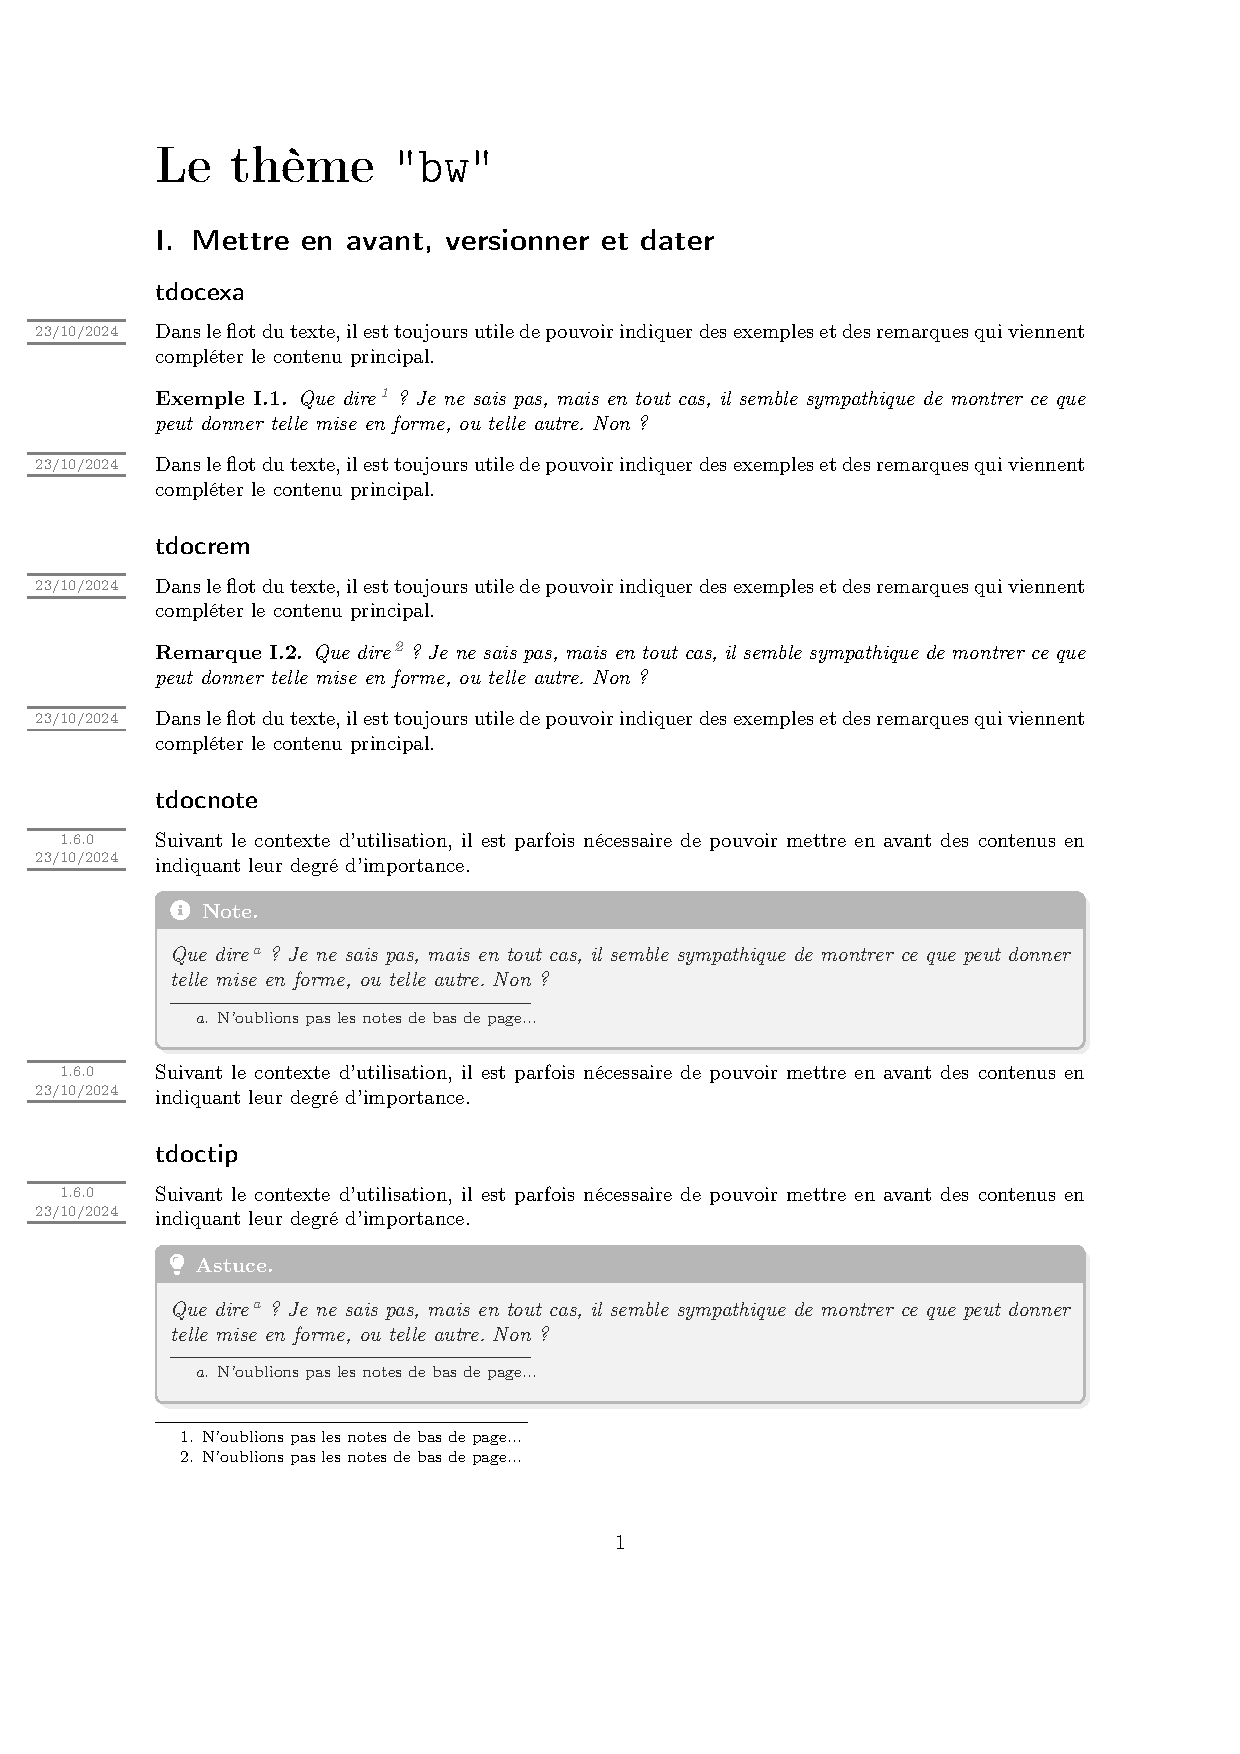
\includepdf[
	pages=1-2,
	fitpaper=true
]{gallery-showcase-bw}

\includepdf[
	pages=1-2,
	fitpaper=true
]{gallery-showcase-color}

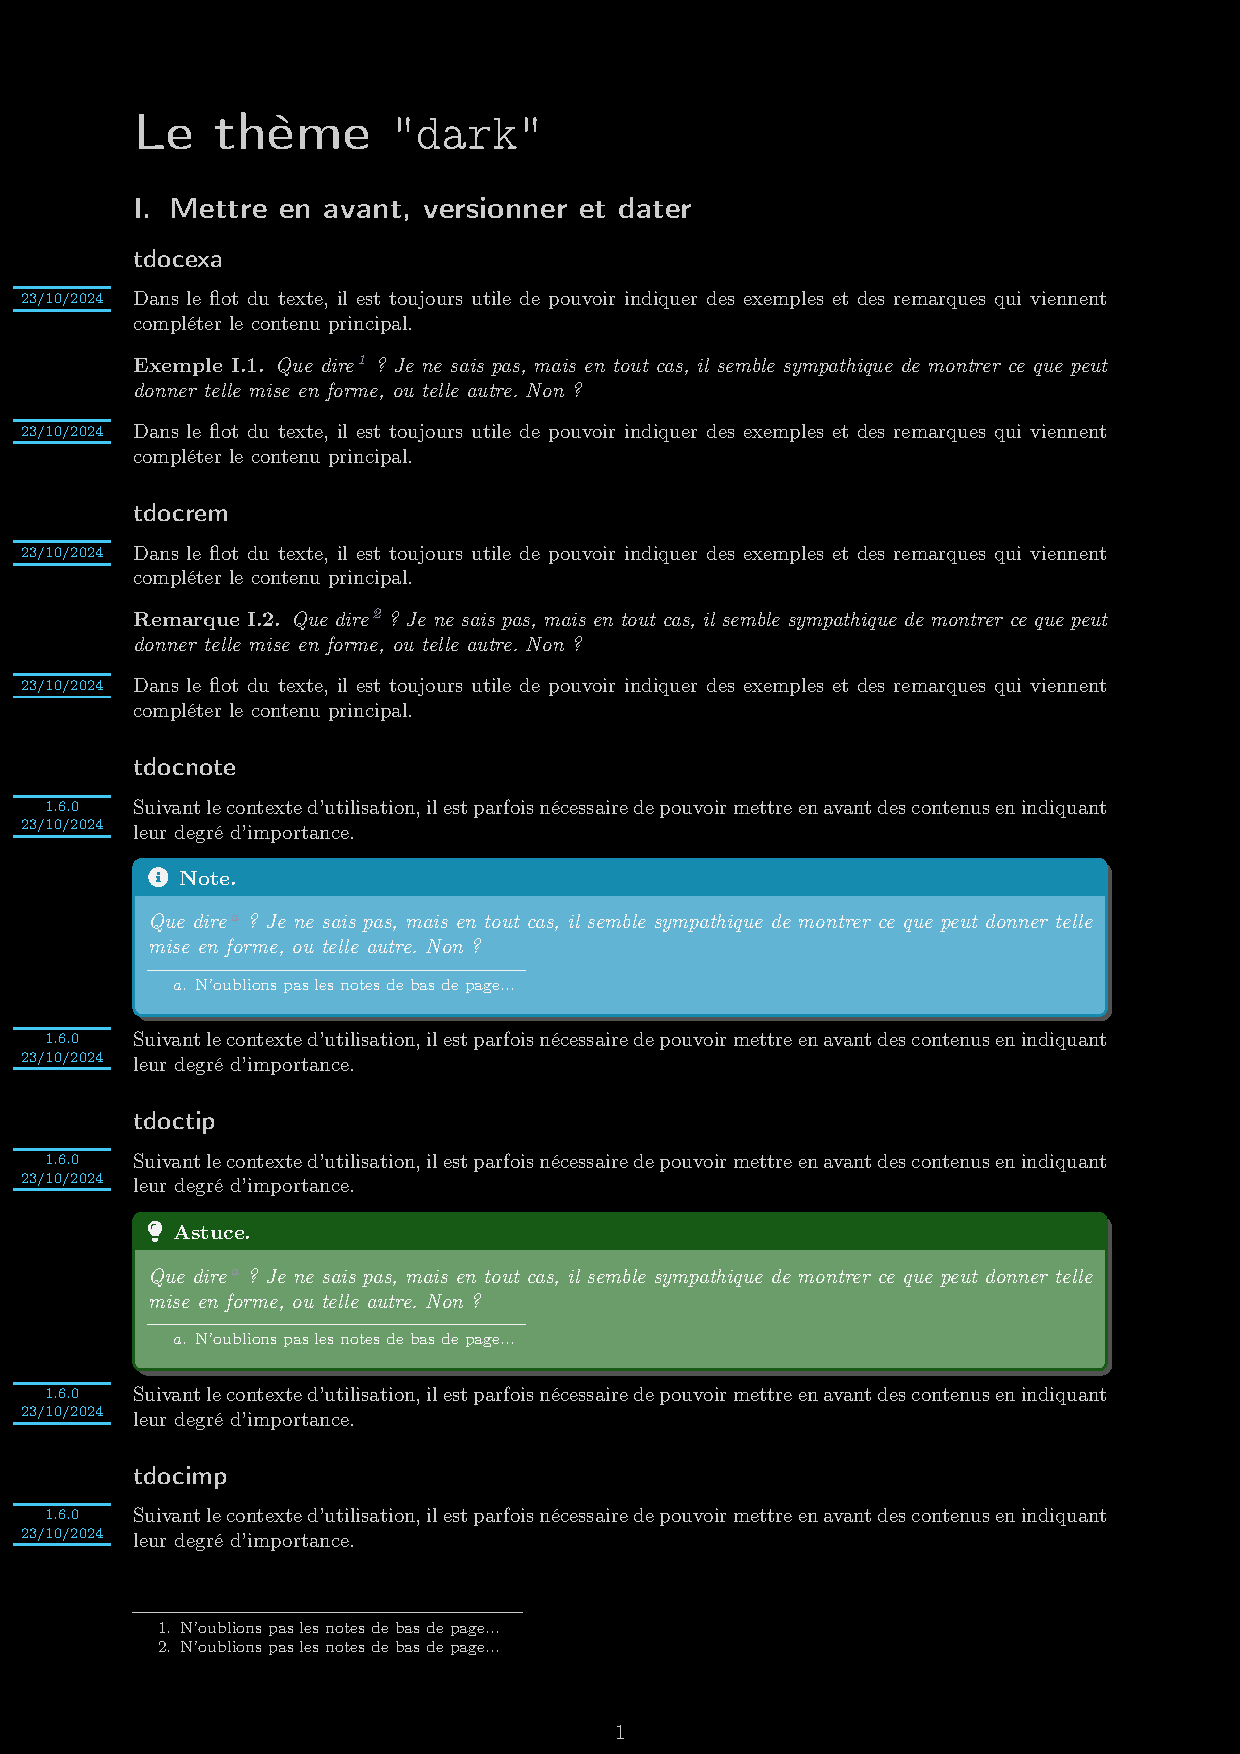
\includepdf[
	pages=1-2,
	fitpaper=true
]{gallery-showcase-dark}

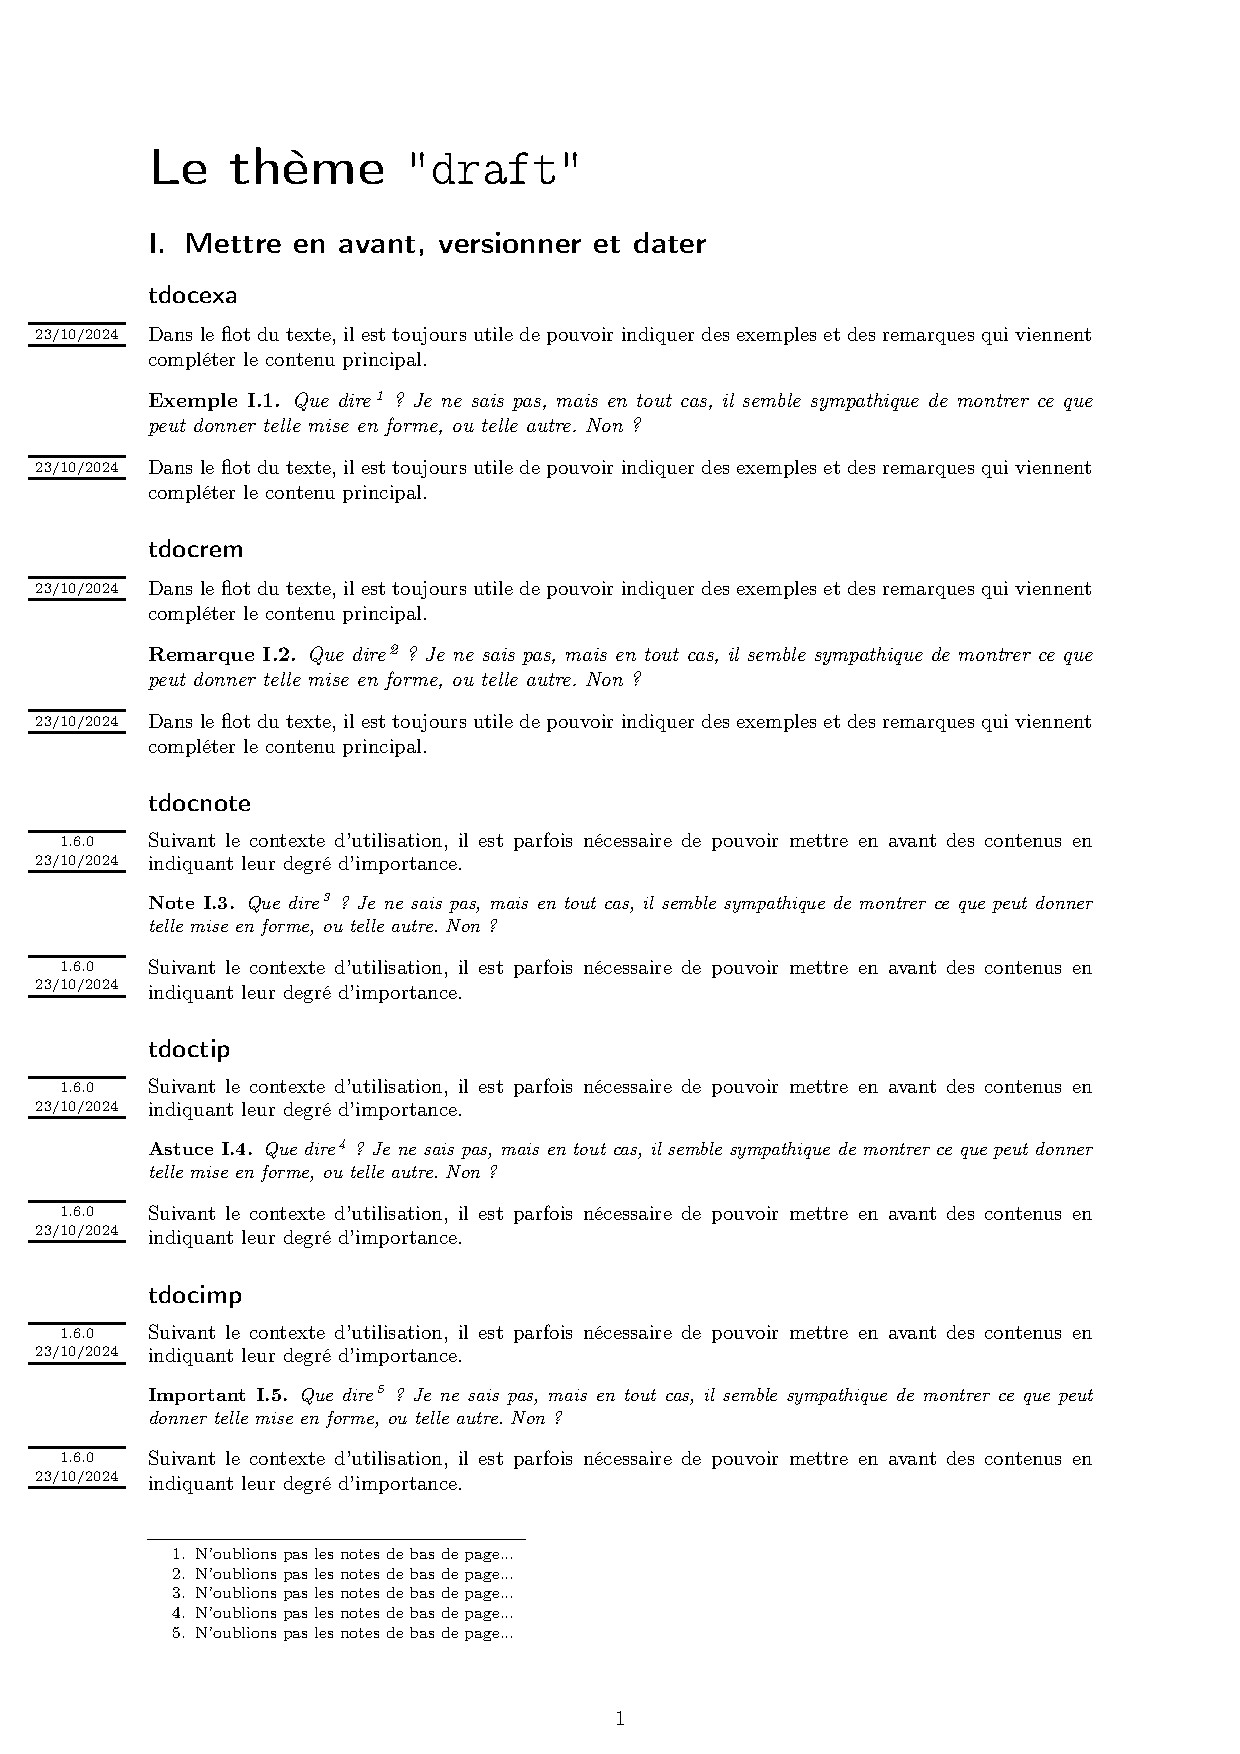
\includepdf[
	pages=1-2,
	fitpaper=true
]{gallery-showcase-draft}

} % AT-END-DOCUMENT - END

\end{document}